\documentclass[10pt]{article}

%------------------------------------------------------
%   PACKAGES
%------------------------------------------------------

% Default 
\usepackage{graphicx}
\usepackage[backend=biber,
  style=numeric, 
  sorting=none]{biblatex}

% Additional
\usepackage{amsmath}
\usepackage{textcomp, gensymb}
\usepackage{placeins}
\usepackage{tabularray} 
\usepackage{xcolor}
\usepackage{placeins}
\usepackage{todonotes}

\newcommand{\td}[1]{\todo[linecolor=blue, backgroundcolor=blue!25,bordercolor=blue, size=\small]{#1}}

\addbibresource{references.bib}

\title{Microwave Optics I} 
\author{Rahmanyaz Annyyev, Hikmat Gulaliyev} 
\date{17 March 2024} 

\begin{document}

\maketitle

\begin{abstract}
In this experiment, we inquire into the wave nature of microwaves. It is divided into three parts, and in each part, we address a different question. First, we determine the wavelength of microwaves using the standing wave pattern. Second, we measure the speed of microwaves in a dielectric material. This is done by measuring the phase shift caused by the material's refractive index. Finally, we investigate a method for generating circularly polarized microwaves from a linearly polarized beam. This is accomplished by manipulating the polarization of the transmitted wave and utilizing a reflecting metal plate with a polarization grille. The results are mostly in line with the theory, except for the third part where there are discrepancies.
\end{abstract}

\section{Introduction}

The electromagnetic spectrum is the range of all possible frequencies of electromagnetic radiation. The spectrum is divided into several regions, in order of decreasing frequency and increasing wavelength: gamma rays, X-rays, ultraviolet, visible light, infrared, microwaves, and radio waves. The microwave region of the electromagnetic spectrum is usually defined as being the range of frequencies from 1 GHz to 100 GHz. The wavelengths of microwaves are usually measured in centimeters. Microwaves are widely used in modern technology, for example in telecommunications, radar, and microwave ovens. The primary goal of this experiment is to verify the wave nature of microwaves \cite{Giancoli_2020}.

The experiment is divided into three parts: A, B, and C. The experimental setup is comprised of a microwave transmitter with a Gunn diode, a microwave receiver with a Schottky diode, a goniometer, three dielectric Perspex\textsuperscript{\textregistered} blocks, a metal reflector, and a polarization grille.

Standing waves are a type of wave that occurs when two waves of the same frequency and amplitude travel in opposite directions and interfere with each other. They are characterized by nodes and antinodes. A node is a point on a standing wave where the wave has zero amplitude. An antinode is a point on a standing wave where the amplitude is at a maximum. The distance between two consecutive nodes or antinodes is equal to half the wavelength of the wave and is denoted by $\lambda/2$ \cite{Sears_&_Zemansky_2013}. In part A of the experiment, we employ this property of standing waves to measure the wavelength of microwaves. The experimental setup is shown in Figure~\ref{fig:1}. We use a microwave transmitter and receiver to detect the standing waves and then measure the distance between two consecutive antinodes to determine the wavelength of the microwaves. The data is taken several times and the average value is found using the formula
\begin{equation}\label{eq:average-wavelength}
  \bar{\lambda} = 2 \frac{\sum\left|x_{i+1}-x_1\right|}{N-1},
\end{equation}
where $x_i$ is the distance between the $i$th antinode and the first antinode, and $N$ is the number of measurements.

\begin{figure}[ht]
  \centering
  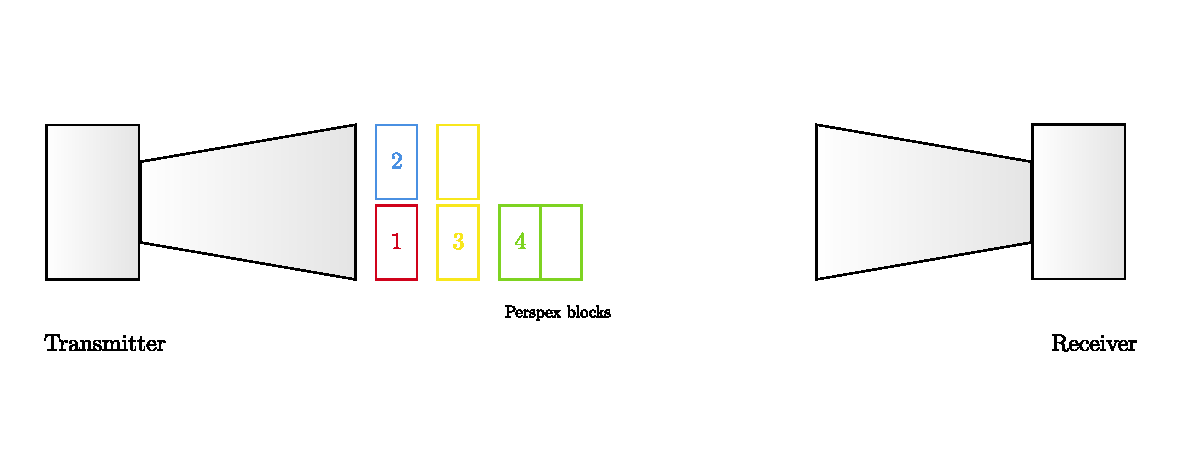
\includegraphics[scale=0.4]{figures/f1.pdf}
  \caption{Experimental setup for part A.}
  \label{fig:1}
\end{figure}

The speed of electromagnetic wave propagation in vacuum is denoted by $c$ and is approximately $3 \times 10^8$ m/s. As the wave enters a dielectric material, the speed of propagation decreases. This is due to the interaction of the electromagnetic wave with the atoms and molecules of the material; the electric and magnetic fields of the wave cause the charges in the material to move, which in turn generates new electromagnetic waves. The superposition of the original wave and the new waves results in a decrease in the progression speed. The speed of propagation in a dielectric material is denoted by $v$ and is given by the equation
\begin{equation}
  v = \frac{c}{n},
\end{equation}
where $n$ is the refractive index of the material. In part B of the experiment, we use a dielectric material to reduce the speed of propagation of microwaves and measure it. The setup is shown in Figure~\ref{fig:2}. In the 4\textsuperscript{th} configuration, there is a phase difference between the waves that affect the intensity. However, it is not equal to $\pi$, so there is no destructive interference. 

\begin{figure}[ht]
  \centering
  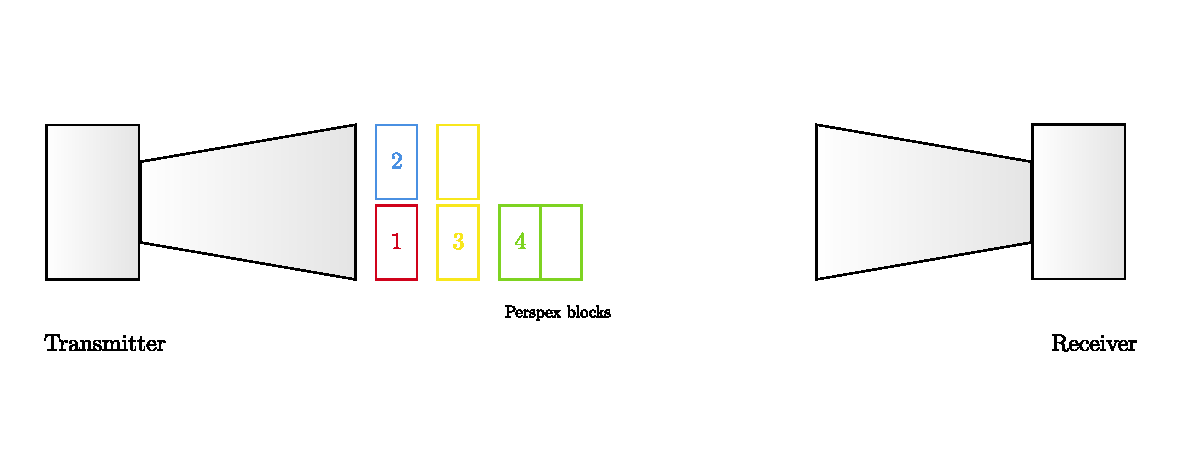
\includegraphics[scale=0.4]{figures/f2.pdf}
  \caption{Experimental setup for part B.}
  \label{fig:2}
\end{figure}

The polarization of an electromagnetic wave is the orientation of the electric field vector. The polarization of a wave can be linear, circular, or elliptical. In part C of the experiment, we use a polarization grille to change the polarization of microwaves and measure the effect of the grille on the intensity of the microwaves. The setup is shown in Figure~\ref{fig:3}. 

\begin{figure}[ht]
  \centering
  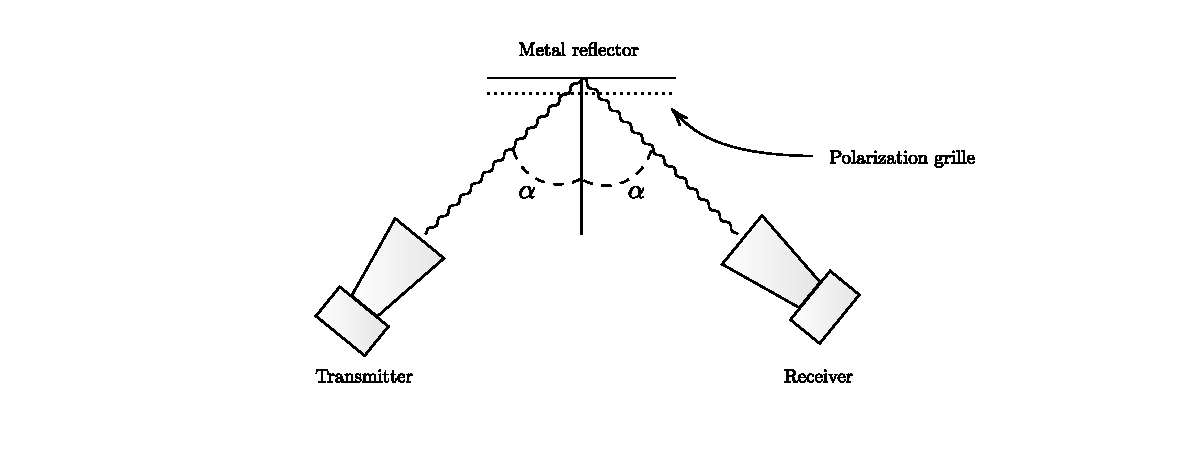
\includegraphics[scale=0.6]{figures/f3.pdf}
  \caption{Experimental setup for part C.}
  \label{fig:3}
\end{figure}

\section{Data \& Results}

The results of part A are shown in Table~\ref{tab:1}. Using Formula~\ref{eq:average-wavelength}, the average value of the wavelength of microwaves is found to be $\bar{\lambda} = 2.925$ cm.

\begin{table}[ht]
  \label{tab:1}
  \centering
  \vspace{4mm}

  \begin{tblr}{
    cells = {halign = c, valign = m},
    row{odd} = {bg = lightgray!5},
    row{1} = {bg = lightgray!20},
    hlines = {},
    vlines = {}
  }
    $i$ & 1 & 2 & 3 & 4 & 5 & 6 & 7 & 8 & 9 \\
    $x_i$ (cm) & 94 & 92.5 & 91.5 & 89.5 & 88 & 86.7 & 85.3 & 83.7 & 82.3 
  \end{tblr}
  \caption{Data for standing waves, part A.}
\end{table}

In part B of the experiment, zero intensity was measured in configurations 1 and 2. The width of a single Perspex\textsuperscript{\textregistered} block is measured to be $L = 2.45$ cm. The refractive index is found the following way:
\begin{align}
  &L(n-1) \cong \dfrac{\lambda}{2}, \\ 
  &n \cong 1 + \dfrac{\lambda}{2L}, \\ 
  &n = 1 + \dfrac{2.925}{2 \cdot 2.45} = 1.59.
\end{align} 
Using this value of $n$, the speed of microwaves in Perspex\textsuperscript{\textregistered} is found to be $v = \frac{c}{n} = \frac{3\times 10^8}{1.59} = 1.89\times 10^8$ m/s. In configurations 3 and 4, there was a drop in intensity. However, since in configuration 3 both parts of the wave pass through the block there wasn't any interference, but some phase shift.  

The results of part C are shown in Table~\ref{tab:2}. The "All" means that the intensity was the same for all settings.

\begin{table}[ht]
  \label{tab:2}
  \centering
  \vspace{4mm}

  \begin{tblr}{
    cells = {halign = c, valign = m},
    row{odd} = {bg = lightgray!5},
    row{1} = {bg = lightgray!20},
    hlines = {},
    vlines = {}
  }
    Receiver angle, $\theta$ & 0\degree & 45\degree & 90\degree & 135\degree & 180\degree & 225\degree & 270\degree & 315\degree \\
    Intensity, $I$ & 0.5 & 0.4 & 0.3 & 0.2 & 0.1 & 0.2 & 0.3 & 0.4 \\
    Setting & $10\times$ & $30\times$ & $30\times$ & All & $10\times$ & $3\times$ & $30\times$ & All
  \end{tblr}
  \caption{Data for polarization, part C.}
\end{table}

\section{Discussion \& Conclusion}

There are several sources of error in part A of the experiment. First, the manual measurement of the distance between antinodes. Second, the use of a ruler to measure the distance. A more precise tool could be used to reduce this error. Third, the horizontal movement of the receiver. The receiver is not fixed in place, so it moves perpendicular to the measurement axis, which introduces errors in the measurements. In part B, the interference pattern is clear as the intensity drops to less than 1 percent of the initial value. However, the Perspex\textsuperscript{\textregistered} blocks have some impurities inside, which change the intensity by moving them. In part C, extensive errors were introduced by unsteady setup. The polarization plate was not fixed relative to the reflector, and the distance between it varied between 3 and 5 centimeters. This issue rendered this part of the experiment unsuccessful. Throughout the experiment, it was assumed that the refractive index of air is 1, and the Perspex\textsuperscript{\textregistered} blocks are uniform and in perfect shape. These assumptions introduce some errors, but they are negligible in this case. In parts A and B, the results are mostly in line with the theory with slight discrepancies. The wavelength of microwaves is found to be $\lambda = 2.925$ cm, and the theoretical value is approximately 2.8cm. The reflection was found to be $n = 1.59$, and the theoretical value is approximately 1.5. It was expected to not get any zero intensity points in part C, which wasn't the case. In general, the experiment was successful in calculating the wavelength of microwaves and refractive index of the Perspex\textsuperscript{\textregistered} blocks but failed to generate circularly polarized microwaves from a linearly polarized beam.

\section{Real World Applications}

While the described experiment focuses on measuring properties and manipulating microwaves in a controlled setting, the underlying principles and setup translate to various real-world applications. A significant example lies in the realm of industrial quality control, particularly for food production. Maintaining consistent moisture content is crucial for the quality, shelf life, and taste of products like bread, cereals, and potato chips. Traditional methods for moisture measurement can be time-consuming or destructive (requiring sample drying). Microwave technology offers a non-destructive and rapid solution.

Similar to the experiment's setup, a metal chamber called a cavity resonator is employed. This chamber resonates at a specific microwave frequency when empty. When a food sample, like a slice of bread, is introduced, the water molecules within it absorb microwave energy, dampening the overall energy. This presence of water alters the electrical properties inside the cavity, causing a shift in its resonant frequency. The extent of this frequency shift is directly proportional to the moisture content. By calibrating the system with samples of known moisture content, this shift can be used to estimate the moisture content of unknown samples quickly and non-destructively. This approach offers significant benefits for production lines, allowing for real-time monitoring and adjustments to maintain consistent product quality.

\printbibliography

\end{document}